\section{MVC Framework}
\label{sec:mvc}
The Model-View-Controller (MVC) was originally designed by Trygve M. H. Reenskaug in 1979, who was at that time working for Xerox PARC. The goal was to create an envoirontment in which the users (developer, customer ect.) could preserve the original perception of the datastructure, while being able to view and edit portions of it.

\subsection{Components}

The (MVC) framework consists of three different types of components; Views, controllers and models. Each created with a different purpose, see figure \ref{fig:mvc-drawing}

\begin{figure}[h]
	\centering
		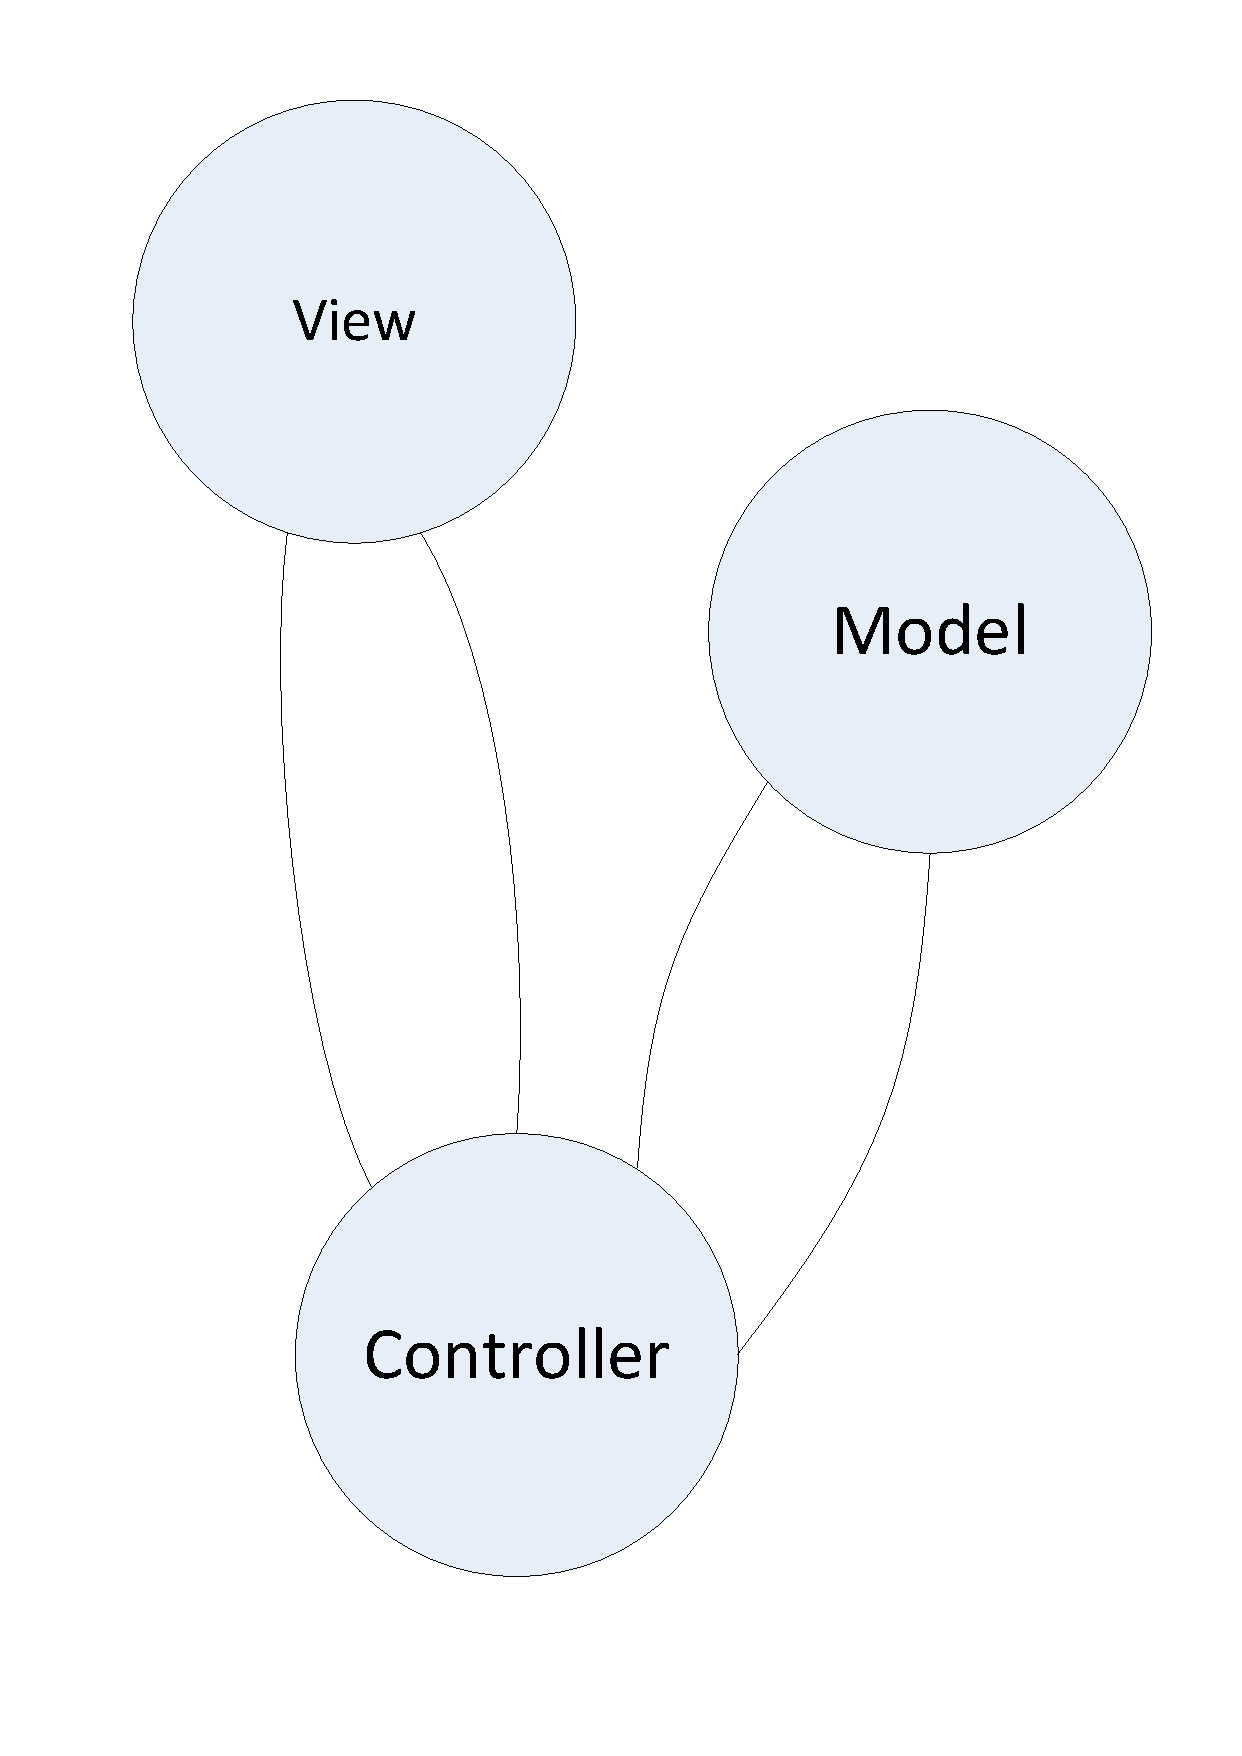
\includegraphics[width=0.90\textwidth]{input/implementation/mvc/MVC.pdf}
	\morscaption{These are the three main components in the MVC}
	\label{fig:mvc-drawing}
\end{figure}


\begin{itemize}
\item Models
\end{itemize}
The models are the components that handle the data domain of the application. The model can be mapped to a database, from which it reads and writes data. This way developers can handle the data, without worrying about the actual data connection.

\begin{itemize}
\item Views
\end{itemize}
The views display the data and UI. They are typically created with data provided from the model. These views are full-featured (X)HTML, with the addtion of C\# or Basic code, to fetch content from the model.

\begin{itemize}
\item Controllers
\end{itemize}
The Controllers reacts to user requests the users provides through the UI. Based on this they deside which view should be rendered. If the data the view should display does not exist in the model (input, ect.) the controller can also provide this data to the view to display.

\subsubsection{Master-page}
Master-pages is not a part of MVC as a design-idea, it is a component implemented by Microsoft. The master-page is a page that is always loaded when displaying a view. Like the view, it consists of (X)HTML and C\#/Basic, however, it also has content-containers. These containers can be created anywhere on the webpage, and are filled with content by views.

\subsection{Structure}
An interesting thing about MVC is that there are no actual HTML files, all content is generated generically as the users interacts with the diferent components within the webpage. When entering an URL you actually call mothods in controllers, you can even add parameters to the calls. The controllers then redirects you to the correct view based on the input and the method called. The view then executes, which results in a plain webpages that can be displayed in a browser.

Because of the seperation into three independent modules, developers are able to create different parts of the application with different kind of approches, thus enabling them to better manage complexity, create applications with a high maintainability, and create UI that does not have to show the actual datastructure, which can often be confusing for an ordinary user of the webpage.

\subsubsection{Data validation}
Client side validation
Server Side validation

\subsubsection{Testing}
When creating web applications with MVC you have the possibility of creating unit tests to thoroughly test your code. These tests can be automatically generated from within Visual Studio, and run as a seperate function, in order to allow the developer to test for all possible inputs. For a more detailed description of Unit-testing in MVC, look in the section \ref{chap:unittest}

\cite{mvcconcept} \cite{mvcxeroxparc} \cite{aspdotnet}



